\documentclass[10pt, a4paper,openany]{article}
\usepackage[italian]{babel}
\usepackage[T1]{fontenc}
\usepackage[table]{xcolor}
\usepackage{float}
\restylefloat{table,figure}
\usepackage{graphicx}	
\usepackage[utf8]{inputenc}
\usepackage{amsmath}
\usepackage{fancyhdr}
\usepackage{geometry}
\geometry{a4paper,top=2cm,bottom=2cm,left=2.5cm,right=2.5cm,%
	    heightrounded,bindingoffset=5mm}
\usepackage{amssymb}
\usepackage{amsthm}
\usepackage{multicol}
\usepackage{xcolor}
\usepackage{hyperref}
\usepackage{caption}
%\usepackage{url}
%inizia qui aggiunta
\usepackage{collcell}
\usepackage{hhline}
\usepackage{pgf}
\usepackage{multirow}
\usepackage{fancyvrb}
\usepackage{verbatim}


\begin{document}
\begin{center}
{\Large\textbf{Guida operativa}}
\end{center}

\begin{center}
 Federico Luzzi,  Marco Peracchi, Christian Uccheddu, Gabriele Centemeri (TTC)
\end{center}
Di seguito la guida operativa per eseguire il codice e replicare i risultati ottenuti:

\section*{Presa dati Dicembre-Gennaio}

Eseguire il file che esegue richieste ogni 30 minuti e salva i dati in formato csv. 

\begin{verbatim}
scraper/scraper_csv.py
\end{verbatim}

Il jupyter-notebook serve a selezionare prese dati ogni 6 ore, e si trova all'interno della cartella \textit{clean\_store\_data}.

\begin{verbatim}
clean_jen_video/fix_jen_json.ipynb
\end{verbatim}

Per trasformare i dati da formato csv a json.

\begin{verbatim}
csv_to_json/main.py
\end{verbatim}

Lo script ha bisogno del parametro:

\begin{itemize}
	\item -d "directory\_dei\_dati"
\end{itemize}

In tal modo si indica la directory dove sono i dati da trasformare.
Per caricare i json su MongoDB avviare lo script:

\begin{verbatim}
json_to_mongo(windows)/json_to_mongo.py
\end{verbatim}

A questo script vanno forniti i seguenti parametri:

\begin{itemize}
	\item -d "directory dei dati"
	\item -u "utente mongo"
	\item -p "password utente"
	\item -port "porta in cui è attivo mongoDB"
	\item-db "nome del database mongo"
	\item -c "collection in cui vengono inseriti i dati"
\end{itemize}


\section*{Presa dati Marzo-Maggio}

Aprire il servizio MongoDB, zookeeper e conseguentemente Kafka. Eseguire in due terminali separati secondo il seguente ordine gli script:

\begin{enumerate}
	\item \begin{verbatim}
	scraper/scraper_consumer.py
	\end{verbatim}
	\item \begin{verbatim}
	scraper/scraper_producer.py
	\end{verbatim}
\end{enumerate}

Ogni 6 ore il \textit{producer} effettua le richieste dati che invia poi al canale Kafka letto dal \textit{consumer} che si occupa della pulizia e immagazzinamento dei dati.

\section*{Presa dati Covid}

Scaricare i dati in formato csv da \href{https://ourworldindata.org/coronavirus-testing}{OurWorldInData}
ed eseguire il codice:

\begin{verbatim}
covid/cleaner.py
\end{verbatim}

Questo script permette di eseguire una pulizia dei dati in modo da renderli integrabili con i json dei video precedenti.

\section*{Integrazione dei dati}


Per eseguire l'integrazione tra i dati Covid e i dati di Youtube bisogna eseguire il seguente script:

\begin{verbatim}
json_to_mongo(windows)/merge_to_mongo.py
\end{verbatim}

A questo script vanno forniti i seguenti parametri:

\begin{itemize}
	\item -d "directory dei dati"
	\item -u "utente mongo"
	\item -p "password utente"
	\item -port "porta in cui è attivo mongodb"
	\item-db "ome del database mongo"
	\item -c "collection in cui vengono inseriti i dati"
	\item -e "path dove c'è file dell'espressione regolare"
\end{itemize}

I dati vengono quindi integrati sulla data e il paese e successivamente caricati su Mongo.

\section*{Query mongo}

La seconda domanda di ricerca ci chiede di distinguere quali video riguardino il coronavirus o meno. L'espressione regolare seguente analizza tags e titoli per verificare se è presente una parola riferita alla pandemia.

\begin{figure}[H]
	\centering
	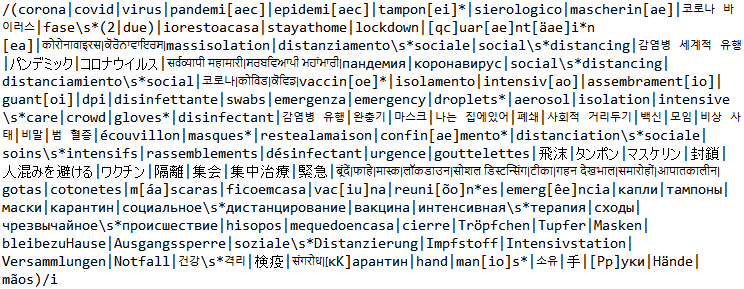
\includegraphics[height=0.4 \linewidth]{er.png}
	\caption{Regular expression usata}
\end{figure}

Per applicare la query sui documenti si possono eseguire singolarmente i comandi in una shell mongo, come viene descritto qui di seguito, oppure è possibile chiamare una funzione che esegue automaticamente tutte e tre le query. 

Eseguire ora i seguenti comandi all'interno della shell di MongoDB.

Creare due nuovi campi chiamati \textbf{covid\_title} e \textbf{covid\_tags} inizializzati entrambi a \textbf{False} 

\begin{Verbatim}[frame=single,baselinestretch=0.1]
db.video_merge.update({},{$set : {covid_tags : false, 
			covid_title : false}},
			{multi : true})
\end{Verbatim}
Eseguire le seguenti due query che controllano se l'espressione regolare è presente nel campo title o in uno dei tag per ogni video.

\begin{Verbatim}[frame=single,baselinestretch=0.1]
db.video_merge.update({tags : {$in : [REGEX]}}, 
			{$set : {covid_tags: true}}, 
			{multi : true})
\end{Verbatim}
 \begin{Verbatim}[frame=single,baselinestretch=0.1]
db.video_merge.update({title : {$in : [REGEX]}}, 
			{$set : {covid_title: true}}, 
			{multi : true})
\end{Verbatim}

\`E possibile eseguire da file le precedenti espressioni, attraverso lo script \textit{query\_covid.py}. Esso viene chiamato come funzione esterna \textit{compute\_covid} durante l'integrazione nello script \textit{merge\_to\_mongo.py} automaticamente.

\section*{Sharding}

Lo sharding dei documenti di Mongo è stato eseguito in locale, quindi utilizzando \textit{localhost} come host. All'interno della cartella \textit{sharding} è possibile visualizzare le cartelle contenenti i vari file di configurazione per tutti i componenti.

\begin{itemize}
	\item \textbf{configsvr} Sono tre istanze di \textit{mongod}, configurate come replica set. Il \textit{config server} conosce dove ogni dato è allocato dei vari shard, quindi è importante configurarlo come replica-set, così che in caso di guasti non si perdano le informazioni.
	\item \textbf{router} \`E un'istanza di \textit{mongos}. Per interrogare i vari shard è necessario interfacciarsi con essa.
	\item \textbf{shard} Sono tre istanze di \textit{mongod}. Ogni shard è configurato in replica-set, e i dati vengono suddivisi nei vari shard.
\end{itemize}

All'interno di ogni cartella sono presenti i vari file di configurazione, dove deve essere specificato il percorso della cartella \textit{data} di ogni istanza. Inoltre bisogna specificare che, essendo configurato tutto in una macchina locale, è importante utilizzare porte differenti per ogni istanza.
\\
Per prima cosa inizializzare i replica-set, e successivamente avviarli come shard server o come config server. Una volta collegati quest'ultimi al router è necessario caricare i dati su uno degli shard. Prima di effettuare la procedura va specificata la \textit{shard key}, e va anche specificato il metodo di suddivisione dei dati, se \textit{hashed} o \textit{ranged}. In questo lavoro è stato utilizzato il primo metodo.
\\
Le collezioni che abbiamo shardato sono state due, una contenente i dati di marzo-maggio integrati con i dati Covid, e l'altra contenente i video di dicembre-gennaio e marzo-maggio. I dati vengono caricati attraverso il router sugli shard, specificando la shard key, e automaticamente suddivisi.

Per ulteriori informazioni sui comandi leggere l'appendice.

\section*{Appendice}

\subsection*{Sharding}

\paragraph{Creazione Config Server\\}
Vengono configurati i tre config server:
\begin{Verbatim}
	mongod --config <file.cfg> --configsvr
\end{Verbatim}

Eseguire il comando sul config server PRINCIPALE, vengono indicati i tre membri del replica set, il quale nome sarà rs0:
\begin{Verbatim}
rs.initiate({ _id: "rs0", 
configsvr: true, members: [{ _id : 0, host : "localhost:27019" },
{ _id : 1, host : "localhost:27020" },
{ _id : 2, host : "localhost:27021" }
]})
\end{Verbatim}

\paragraph{Creazione Shard Server\\} Aprire tutte le istanze di mongod dei vari shard.

\begin{Verbatim}
mongod --config <file.cfg> --shardsvr
\end{Verbatim}

Successivamente per ogni gruppo replica-set accedere ad uno ed inizializzare il gruppo:
\begin{itemize}
	\item Primo gruppo
\begin{Verbatim}
rs.initiate(
{_id : "rs1",
members: [
{ _id : 0, host : "localhost:27022" },
{ _id : 1, host : "localhost:27023" },
{ _id : 2, host : "localhost:27024" }
]
}
)
\end{Verbatim}
	\item Secondo Gruppo
\begin{Verbatim}
rs.initiate(
{_id : "rs2",
members: [
{ _id : 0, host : "localhost:27025" },
{ _id : 1, host : "localhost:27026" },
{ _id : 2, host : "localhost:27027" }
]
}
)
\end{Verbatim}

	\item Terzo gruppo
\begin{Verbatim}
rs.initiate(
{_id : "rs3",
members: [
{ _id : 0, host : "localhost:27028" },
{ _id : 1, host : "localhost:27029" },
{ _id : 2, host : "localhost:27030" }
]
}
)
\end{Verbatim}

\end{itemize}

\paragraph{Router\\}
Dopo aver inizializzato gli shard e i config server aprire il router come istanza di mongos:

\begin{Verbatim}
mongos --config <file.cfg>
\end{Verbatim}

Dopo aver avviato il router connettersi ad esso attraverso il localhost e la porta ad esso associata mediante il comando:

\begin{Verbatim}
mongo --host <router>
\end{Verbatim}

Ora è possibile aggiungere i vari shard mediante il comando \textit{sh.addShard()} al router, inserendo tra le parentesi l'indirizzo di collegamento allo shard. Nel nostro caso, avendo impostato come replica-set ogni shard è necessario utilizzare:
\begin{itemize}
	\item Primo shard
	\begin{Verbatim}
	sh.addShard("rs1/localhost:27022,localhost:27023,localhost:27024")
	\end{Verbatim}
	\item Secondo shard
	\begin{Verbatim}
	sh.addShard("rs2/localhost:27025,localhost:27026,localhost:27027")
	\end{Verbatim}
	\item Terzo shard
	\begin{Verbatim}
	sh.addShard("rs3/localhost:27028,localhost:27029,localhost:27030")
	\end{Verbatim}
\end{itemize}

Adesso è possibile caricare i dati mediante il router mongos e applicare lo shard, utilizzando come chiave il paese. Il comando da utilizzare è:

\begin{Verbatim}
sh.shardCollection("YT_data.video_all", {country_name : "hashed"})
\end{Verbatim}

La collezione risulta ora distribuita su tre shard, tutti configurati come replica-set.

\subsection*{Versione Software}
Le versioni utilizzate
\begin{itemize}
	\item \textbf{Zookeeper} 3.4.10
	\item \textbf{Apachi Kafka} 2.3.0
	\item \textbf{MongoDB} 4.2
	\item \textbf{Python} 3.6
	\item \textbf{Tableau} 2019.4.7
\end{itemize}



\end{document}


